\chapter{Συστήματα Peer-to-Peer}
\label{chap:P2P}

\section{Εισαγωγή}

Ένα peer-to-peer σύστημα είναι ένα δίκτυο αποτελούμενο από ισότιμους 
συμμετέχοντες, τους peer. Αυτοί διαμοιράζονται τους πόρους που έχει ο 
καθένας μεταξύ τους, όπως υπολογιστική ισχύ ή αποθηκευτικό χώρο. 
Χαρακτηριστικό του συστήματος, που το διαχωρίζει από την κλασική 
αρχιτεκτονική client-server, είναι πως ένας peer είναι πάροχος υπηρεσιών 
και πόρων και την ίδια στιγμή αιτείται αντίστοιχη χρήση από 
απομακρυσμένους peer. Τα peer-to-peer συστήματα χωρίζονται σε δομημένα 
(structured) και μη (unstructured). 

Στα δομημένα peer-to-peer συστήματα η τοπολογία του δικτύου 
κατασκευάζεται ντετερμινιστικά με μια κλασική οργάνωση να είναι οι 
κατανεμημένοι πίνακες κατακερματισμού (DHT). Υπάρχει ένας ευρύτερος 
χώρος αναγνωριστικών από όπου τα δεδομένα και οι peer αντιστοιχούνται σε 
κλειδιά. Ένα σημαντικό ζήτημα του συστήματος είναι για ποια δεδομένα 
είναι υπεύθυνος ένας peer βάσει των κλειδιών τους. Παράδειγμα τέτοιου 
συστήματος είναι το Chord \citep{Tanenbaum2006}. Οι peer οργανώνονται 
πάνω σε ένα κύκλο. Κάθε peer είναι υπεύθυνος για εκείνα τα δεδομένα που 
τους αναλογούν κλειδιά μικρότερα σε σχέση με αυτό του peer. Επίσης, ένας 
peer, με βάση την τοποθεσία του, διατηρεί μια λίστα από γείτονες peer οι 
οποίοι βρίσκονται σε συγκεκριμένες αποστάσεις πάνω στον κύκλο. Το 
αποτέλεσμα αυτής της τοπολογίας του Chord είναι πως ένα lookup 
εξυπηρετείται σε $O(logN)$ βήματα.

Η δεύτερη περίπτωση είναι τα μη δομημένα συστήματα. Αυτά στηρίζονται 
συνήθως σε τυχαιοκρατικούς αλγορίθμους για την κατασκευή της τοπολογίας. 
Δεν υπάρχει ένας συγκεκριμένος σχηματισμός και κάθε peer σχετίζεται με 
γείτονες που έχουν επιλεγεί τυχαία. Μια συνηθισμένη πρακτική σε αυτή την 
κατηγορία συστημάτων είναι η ύπαρξη των υπερκόμβων (supernode). Όσο το 
δίκτυο επεκτείνεται, τόσο περισσότερο αυξάνεται ο χρόνος εξυπηρέτησης 
ενός lookup. Ταυτόχρονα έχουμε και αυξημένη χρήση του bandwidth του 
δικτύου μιας και η πρακτική που ακολουθείται είναι αυτή του flooding. Οι 
υπερκόμβοι λύνουν αυτό το πρόβλημα είτε διατηρώντας ένα ευρετήριο με 
τους πόρους και τους peer του δικτύου είτε λειτουργώντας ως 
διαμεσολαβητές στη δρομολόγηση των μηνυμάτων (broker). Αφού είναι και 
αυτοί μέρος του δικτύου, τότε το σύστημα οδηγείται σε μια ιεραρχική 
δομή.

\section{Το P-Grid Σύστημα}

Το P-Grid 
\citep{Abererb, Aberer, Abererc, Abererd, Aberer2004, Aberer2003, Aberere, Aberer2002} 
είναι ένα πλήρως αποκεντρωμένο και δομημένο 
(structured) peer-to-peer σύστημα. Χρησιμοποιεί τυχαιοκρατικούς 
αλγορίθμους για την κατασκευή και την λειτουργία του. Η τοπολογία που 
δημιουργείται είναι ένα δυαδικό trie δέντρο και χρησιμοποιούνται 
προθέματα κλειδιών για την δρομολόγηση των μηνυμάτων μέσα στο δίκτυο.

Οι peer αποφασίζουν κατά ζεύγη τον τρόπο με τον οποίο θα 
χωρίσουν το χώρο κλειδιών (key space). Κάθε κατάτμηση του χώρου 
αντιστοιχεί σε μια συγκεκριμένη δυαδική συμβολοσειρά ή οποία αποτελεί 
και το μονοπάτι ενός peer. Στο σχήμα \ref{fig:PGrid_overlay} φαίνεται η τελική 
διαμόρφωση του χώρου κλειδιών και της τοπολογίας που έχουν σχηματίσει οι 
peer. Το δίκτυο αποτελείται από τέσσερις peer κάθε ένας εκ των οποίων 
έχει συσχετιστεί με ένα μονοπάτι. Η ρίζα του δέντρου αποτελεί το 
συνολικό χώρο των κλειδιών. Οι διακλαδώσεις σε κάθε ύψος αναπαριστούν 
κατατμήσεις του χώρου ένα ψηφίο τη φορά. Παράδειγμα, μετά τη ρίζα, 
έχουν δημιουργηθεί δύο μεγάλα υπόδεντρα. Το αριστερό περιλαμβάνει όλα τα 
κλειδιά τα οποία έχουν πρόθεμα το \textit{'0'}, ενώ το αριστερό αυτά που έχουν 
πρόθεμα το \textit{'1'}. Συνεπώς, οι peer ανάλογα με το μονοπάτι με το οποίο 
έχουν συσχετιστεί, γνωρίζουν ένα συγκεκριμένο πλήθος κλειδιών.

\begin{figure}[htbp]
\centering
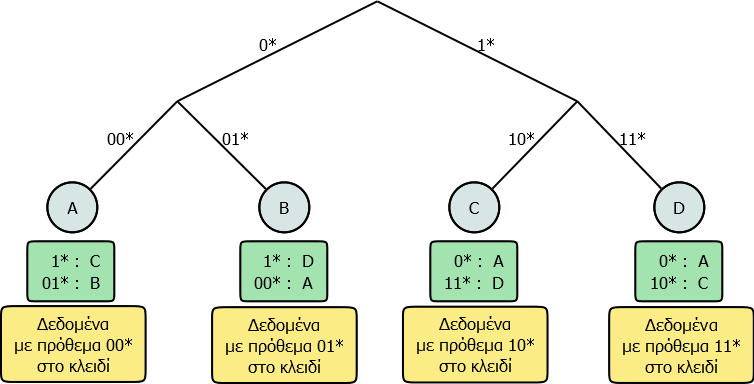
\includegraphics[scale=0.4]{Figures/P2P_PGrid/PGrid_overlay_network.png}
\caption{Η τοπολογία ενός δικτύου P-Grid}
\label{fig:PGrid_overlay}
\end{figure}

Για κάθε επίπεδο του δέντρου, αποθηκεύονται αναφορές στον πίνακα 
δρομολόγησης προς τους peer των οποίων το μονοπάτι ανήκει στο συζυγές 
υπόδεντρο. Παράδειγμα, ο peer Α έχει μονοπάτι \textit{'00'} και επομένως θα 
αποθηκεύσει αναφορές για το επίπεδο με μονοπάτι \textit{'0'} έναν peer από το 
συζυγές του που είναι το υπόδεντρο με μονοπάτι \textit{'1'}. Αντίστοιχα για το 
\textit{'00'} είναι το \textit{'01'}. Στο σχήμα \ref{fig:PGrid_overlay} έχει 
συσχετίσει το \textit{'1'} με τον peer C και το \textit{'01'} με τον B. 
Η επιλογή των peer που θα επιλέξει να κρατήσει αναφορές είναι τυχαία. Επίσης, 
οι peer που αποθηκεύονται ανά επίπεδο μπορεί να είναι περισσότεροι του ενός. 
Βάσει αυτής της τοπολογίας, μια αναζήτηση θα κάνει Ο(logN) βήματα μέχρι να 
βρεθεί το αποτέλεσμα της. Άλλο πλεονέκτημα είναι και η δυνατότητα εκτέλεσης 
αναζητήσεων με δεδομένο ένα εύρος κλειδιών (key range).

Όσον αφορά τα δεδομένα που μπορεί να αποθηκεύσει κάθε peer, 
ακολουθείται η ίδια λογική. Υπάρχει μια συνάρτηση κατακερματισμού η 
οποία αντιστοιχεί κλειδιά σε δεδομένα. Κάθε peer είναι υπεύθυνος για 
εκείνο το κομμάτι των δεδομένων που έχει πρόθεμα το μονοπάτι του.

Τέλος, το σύστημα υποστηρίζει διάφορα πρωτόκολλα. Αυτό που μας 
ενδιαφέρει στην παρούσα εργασία είναι αυτό της ανοχής λαθών 
(fault-tolerance). Αυτό που προτείνεται και είναι ήδη υλοποιημένο είναι 
η τεχνική της αντιγραφής (replication). Κάθε μονοπάτι του δέντρου 
αντιστοιχεί σε πολλαπλούς peer. Αυξάνει τη γενική αντοχή του συστήματος 
σε αποτυχίες peer. Το κόστος είναι η μείωση της χωρητικότητας του 
δικτύου, αφού μέρος των peer είναι αντίγραφα άλλων. Επίσης γίνεται πιο 
πολύπλοκη η διατήρηση και ο συγχρονισμός του συστήματος. 
